\chapter{Question 4}
\section{Questions}
Hughes-Hallett \emph{et al}, 2013. Chapter 4, Section 3, Problem 42: \\
\\
\noindent On the same side of a straight river are two towns, and the
townspeaople want to build a pumping station, $S$. See figure 4.43. The pumping
station is to be at the river's edge with pipes extending straight to the two
towns. Where should the pumping station be located to minimize the total length
of pipe?

\section{Solutions}
County needs to order about 6.4 miles of pipe. An exact value is presented
following verbose working to solutions.

S, Town 1 and Town 2 are awful names. Let Town 1 be North Drysdale and Town 2 be
South Drysdale. Pumping Station will be named the Richard Nixon Pumphouse
\footnote{because it's a watergate!}.\\
\\
\noindent Recognise there are two Pythaorean triads to be formed where the pipe
forms hypotenuse of both triangles to the Watergate Pumphouse. As given in the
diagram, $x$ is the distance the intersection of a due North bearing from North
Drysdale to the river. This yields two distances:
\begin{align}
  \text{North Drysdale pipe}
    &= \sqrt{1+x^2} \\
  \text{South Drysdale pipe}
    &= \sqrt{4^2 + (4-x)^2} \\
    &= \sqrt{16 + (16-8x+x^2)} \\
    &= \sqrt{x^2 -8x +32}
  \intertext{Let Total Pipe be given by the function $p(x)$ such that:}
  p(x) &= \text{Total Pipe} \\
    &= \text{North Drysdale pipe} + \text{South Drysdale pipe} \\
    &= \sqrt{1+x^2} + \sqrt{x^2 -8x +32}
\end{align}
Now we seek global minima of $p(x)$. Using Mathematica, $p(x)$ can be plotted
using the code:\\
\texttt{Plot[Sqrt[1 + x\^{}2] + Sqrt[32 - 8 x + x\^{}2], \{x, -2, 4\},PlotRange $\to$ \{0,10\}, ImageSize
$\to$ Large]}.
\begin{figure}[!h]
  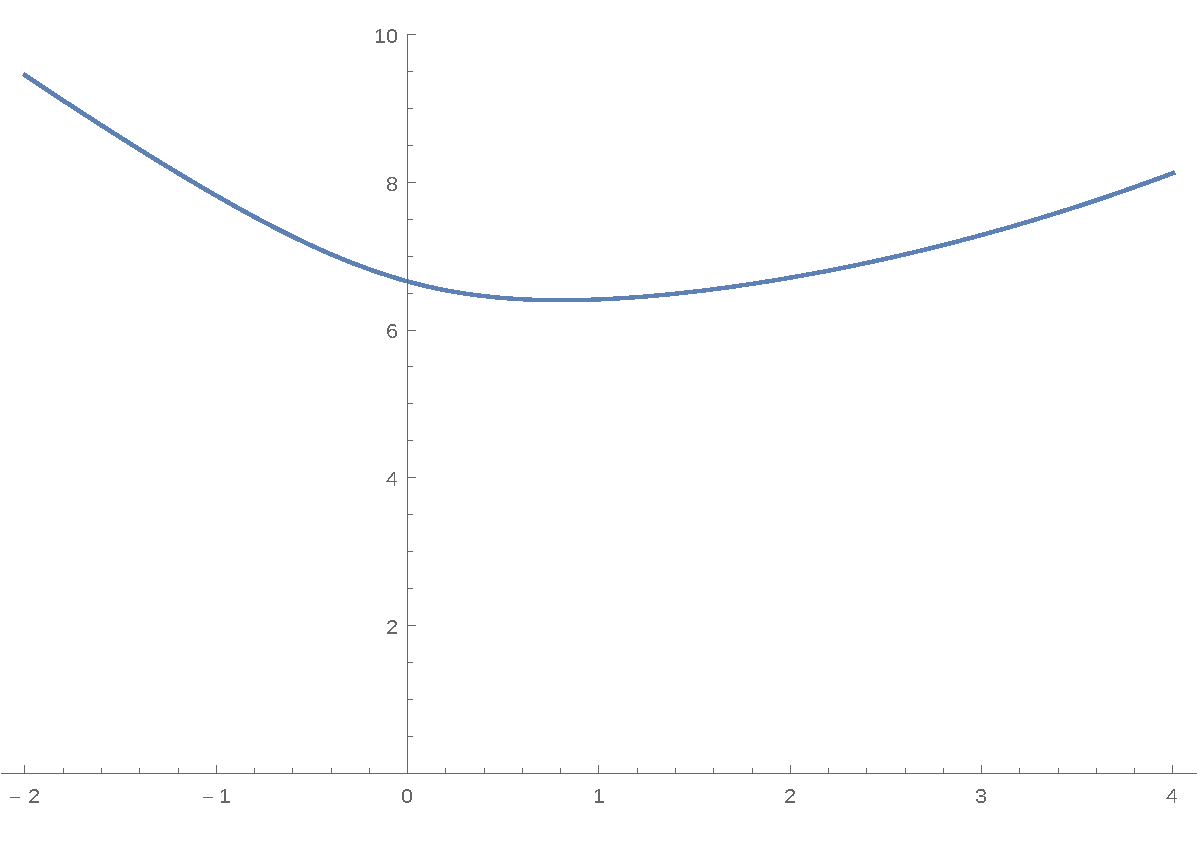
\includegraphics[width=\linewidth]{solutions/q4/plot1.pdf}
  \caption{Plot of $p(x)=\sqrt{1+x^2} + \sqrt{x^2 -8x +32}$}
\end{figure}\\
The minima is somewhere near $x=1$ indicating around 1 mile is good guess, but
a more precise answer can be found if we take find the derivative of $p(x)$,
and then the roots of $p'(x)$ should give us the exact distance for $x$. From
here we can also work out how much pipe is required.\footnote{Apologies if this
appears highly verbose, but I don't understand my own working unless I annotate
it.}
\begin{align}
  p(x) &= \sqrt{1+x^2} + \sqrt{x^2 -8x +32} \nonumber \\
  p'(x)
    &= (\sqrt{1+x^2})' + (\sqrt{x^2 -8x +32})'
  \intertext{Apply chain rule, let $f(x) = \sqrt{x}$ and $g(x)=(1+x^2)$ st}
  (f(x))'
    &= f'(g(x)) \cdot g'(x) \\
    &= \frac{1}{2\sqrt{1+x^2}} \cdot 2x
  \intertext{Apply chain rule, let $f(x) = \sqrt{x}$ and $g(x)=(x^2 -8x +32)$ st}
  (f(x))'
    &= f'(g(x)) \cdot g'(x) \\
    &= \frac{1}{2\sqrt{x^2 -8x +32}} \cdot (2x -8)
  \intertext{Sum both derivatives}
  p'(x)
    &= \frac{1}{2\sqrt{1+x^2}} \cdot 2x
     + \frac{1}{2\sqrt{x^2 -8x +32}} \cdot (2x -8)
  \intertext{Collect like terms}
    &= \frac{2x}{2\sqrt{1+x^2}} + \frac{2x -8}{2\sqrt{x^2 -8x +32}}
  \intertext{Divide out the twos}
    &= \frac{x}{\sqrt{1+x^2}} + \frac{x -4}{\sqrt{x^2 -8x +32}}
  \intertext{Cross multiply to make a single fraction:}
    &= \frac{\left(x\sqrt{x^2-8x+32}\right)+\left((x-4)\sqrt{1+x^2}\right)}{\sqrt{1+x^2}{\sqrt{x^2-8x+32}}}
  \intertext{Since we want the roots, we need to find when $p'(x)=0$}
  0 &= \frac{\left(x\sqrt{x^2-8x+32}\right)+\left((x-4)\sqrt{1+x^2}\right)}{\sqrt{1+x^2}{\sqrt{x^2-8x+32}}} \\
    &= \left(x\sqrt{x^2-8x+32}\right)+\left((x-4)\sqrt{1+x^2}\right) \\
  \left(x\sqrt{x^2-8x+32}\right)
    &= -(x-4)\sqrt{1+x^2} \\
  \left(x\sqrt{x^2-8x+32}\right)^2
    &= \left(-(x-4)\sqrt{1+x^2}\right)^2 \\
  (x^2)(x^2-8x+32) &= (-(x-4))^2(1+x^2) \\
  x^4 -8x^3 +32x^2 &= (x^2-8x+16)(1+x^2) \\
                   &= x^2 -8x +16 +x^4 -8x^3 +16x^2 \\
  15x^2 +8x -16 &= 0 \\
  \intertext{Apply quadratic formula}
  (3x+4)(5x-4) &= 0 \\
  x &= \frac{4}{5} \quad \text{or} \quad \frac{-4}{3}
\end{align}
$\frac{4}{5}=0.8$ miles. The negative solution is discounted because it is west
of North Drysdale and South Drysdale is south-east resulting in more pipe than
necessary.

Finally, the total amount of pipe necessary can be found substituting
$x=\frac{4}{5}$ into the original equation,
\begin{align}
  p(\frac{4}{5}) &= \sqrt{1+\frac{4}{5}^2} + \sqrt{\frac{4}{5}^2 -8\frac{4}{5} +32} \\
  &= \sqrt{41} \\
  &\approx 6.4
\end{align}
About 6.4 miles of pipe needs to be ordered.\footnote{At this point it is
worth noting that only a few metres of pipe need to be ordered if the county
were willing to build viaducts above ground, however this student suspects that
the question would then be changed to minimise viaducts.}\qedbitches
